\documentclass[11pt]{article}

\usepackage[letterpaper,margin=1in]{geometry}
\usepackage[T1]{fontenc}
\usepackage[utf8]{inputenc}
\usepackage{lmodern}
\usepackage{microtype}
\usepackage{amsmath,amssymb,mathtools,bm}
\usepackage{enumitem}
\usepackage{xcolor}
\usepackage{booktabs}
\usepackage{array}
\usepackage{hyperref}
\usepackage[most]{tcolorbox}
\usepackage{fancyhdr}
\usepackage{titlesec}
\usepackage{parskip}
\usepackage{needspace}
\usepackage{pgfplots}
\pgfplotsset{compat=1.18}

\definecolor{qftblue}{HTML}{245A8D}
\definecolor{qftgreen}{HTML}{2F6B4F}
\definecolor{qftred}{HTML}{A23B3B}
\definecolor{qftgray}{HTML}{F4F6F8}

\hypersetup{
  colorlinks=true,
  linkcolor=qftblue,
  urlcolor=qftblue,
  citecolor=qftgreen,
  pdftitle={PHYS 662 Lecture 6: A Few Important Examples},
  pdfauthor={Nima Lashkari}
}

\pagestyle{fancy}
\fancyhf{}
\lhead{PHYS 662: Quantum Field Theory I}
\rhead{Lecture 6}
\cfoot{\thepage}
\setlength{\headheight}{14pt}

\titleformat{\section}{\Large\bfseries\color{qftblue}}{\thesection.}{0.6em}{}
\titleformat{\subsection}{\large\bfseries\color{qftgreen}}{\thesubsection}{0.6em}{}
\titleformat{\subsubsection}{\normalsize\bfseries\color{qftred}}{\thesubsubsection}{0.6em}{}

\setlist[itemize]{leftmargin=2em,itemsep=0.25em,topsep=0.4em}
\setlist[enumerate]{leftmargin=2em,itemsep=0.25em,topsep=0.4em}

\newcommand{\dd}{\mathrm{d}}
\newcommand{\R}{\mathbb{R}}
\newcommand{\Lag}{\mathcal{L}}
\newcommand{\cM}{\mathcal{M}}
\newcommand{\SO}{\mathrm{SO}}
\newcommand{\OO}{\mathrm{O}}

\newtcolorbox{keyidea}[1][]{
  enhanced, breakable, colback=qftgray, colframe=qftblue,
  boxrule=0.8pt, arc=1.5mm, title={#1}, fonttitle=\bfseries,
  coltitle=white
}
\newtcolorbox{remarkbox}[1][]{
  enhanced, breakable, colback=white, colframe=qftgreen,
  boxrule=0.7pt, arc=1.5mm, title={#1}, fonttitle=\bfseries,
  coltitle=white
}
\newtcolorbox{warningbox}[1][]{
  enhanced, breakable, colback=white, colframe=qftred,
  boxrule=0.7pt, arc=1.5mm, title={#1}, fonttitle=\bfseries,
  coltitle=white
}

\begin{document}
\pagenumbering{gobble}
\begin{titlepage}
\centering
\vspace*{1.2in}
{\scshape\Large PHYS 662 --- Quantum Field Theory I\par}
\vspace{0.35in}
{\Huge\bfseries\color{qftblue} Lecture 6\par}
\vspace{0.15in}
{\LARGE\bfseries A Few Important Examples\par}
\vspace{0.12in}
{\Large\color{qftgreen} Scalar Fields, Electromagnetism, and Statistical Fields\par}
\vspace{0.6in}
{\large Nima Lashkari\par}
{\large Fall 2026\par}
\vfill
\begin{minipage}{0.86\textwidth}
\small
We apply the action principle to four examples: the massive relativistic
scalar, the nonrelativistic complex scalar, Maxwell electrodynamics, and a
coarse-grained statistical system. The examples explain how a Lagrangian
encodes a dispersion relation, how first-order dynamics differs from
second-order dynamics, why gauge potentials introduce constraints, and how
coarse-graining generates a symmetry-constrained local action. The final example
introduces Landau's order-parameter paradigm and its Wilsonian extension.

\medskip
Course page: \url{https://nimalashkari.com/quantum-field-theory-2026-part-i/}
\end{minipage}
\vspace{0.5in}
\end{titlepage}
\pagenumbering{roman}
\tableofcontents
\newpage
\pagenumbering{arabic}

\section*{Roadmap}
\addcontentsline{toc}{section}{Roadmap}

Lecture 5 supplied the general variational machinery. Here we use it to
compare theories with different degrees of freedom and different physical
interpretations:
\begin{enumerate}
\item a real relativistic scalar obeys the Klein--Gordon equation;
\item a complex nonrelativistic field obeys a first-order equation with the
same form as the one-particle Schrodinger equation;
\item a gauge potential describes electromagnetism using redundant variables;
\item a block magnetization explains where effective actions come from and
leads to Landau's description of phases and transitions.
\end{enumerate}
The first three examples concern classical real-time dynamics. The fourth
concerns statistical weights. Quantization will give particle interpretations
to the dynamical fields, but a classical field is not already a wavefunction.

\begin{keyidea}[Conventions]
We use \(\hbar=c=1\), \(D=d+1\), and
\(\eta_{\mu\nu}=\operatorname{diag}(1,-1,\ldots,-1)\). Thus
\(\Box=\partial_t^2-\nabla^2\). Our positive-frequency convention is
\(e^{-i\omega t+i\bm k\cdot\bm x}\), with \(\omega>0\).
Electromagnetic component formulas are in \(3+1\) dimensions and rationalized
units. In statistical mechanics we also set \(k_B=1\).
\end{keyidea}

\Needspace{7\baselineskip}
\section{Review: varying a local action}

For fields \(\phi^a\), the action is
\begin{equation}
S[\phi]=\int_\cM\dd^D x\,\Lag(\phi^a,\partial_\mu\phi^a,x).
\end{equation}
Its first variation is the term linear in \(\delta\phi^a\):
\begin{align}
\delta S
&=\int_\cM\dd^D x\left[
\frac{\partial\Lag}{\partial\phi^a}\delta\phi^a+
\frac{\partial\Lag}{\partial(\partial_\mu\phi^a)}
\partial_\mu\delta\phi^a\right]\notag\\
&=\int_\cM\dd^D x\left[
\frac{\partial\Lag}{\partial\phi^a}-
\partial_\mu\frac{\partial\Lag}{\partial(\partial_\mu\phi^a)}
\right]\delta\phi^a
+\int_{\partial\cM}\dd\Sigma_\mu\,
\frac{\partial\Lag}{\partial(\partial_\mu\phi^a)}\delta\phi^a.
\label{eq:variation}
\end{align}
For compactly supported variations, or boundary conditions that remove the
last term, stationarity gives
\begin{equation}
\boxed{\frac{\partial\Lag}{\partial\phi^a}-
\partial_\mu\frac{\partial\Lag}{\partial(\partial_\mu\phi^a)}=0.}
\label{eq:EL}
\end{equation}
Here \(\partial_\mu\) acting on a function of the fields includes their
spacetime dependence. In jet notation this is often denoted \(D_\mu\), a
total derivative. Also,
\(S[\phi+\delta\phi]-S[\phi]=\delta S+O((\delta\phi)^2)\);
the finite difference and the first variation agree only to first order.

\Needspace{7\baselineskip}
\section{Example 1: the massive relativistic scalar}

\subsection{The Lagrangian and Poincare invariance}

Let \(\phi(x)\) be a real scalar. Take
\begin{equation}
\Lag=\frac12\partial_\mu\phi\,\partial^\mu\phi-V(\phi),
\qquad V(\phi)=\frac12m^2\phi^2.
\label{eq:scalarL}
\end{equation}
Under \(x'=\Lambda x+a\), the scalar law is \(\phi'(x')=\phi(x)\).
The metric contraction makes the kinetic term a Lorentz scalar, and
\(\dd^D x'=\dd^D x\). The absence of explicit \(x\)-dependence gives
translation invariance, assuming the integration domain and boundary
conditions transform appropriately. Thus the action is Poincare invariant.

In time and space components,
\begin{equation}
\Lag=\frac12\dot\phi^2-\frac12|\nabla\phi|^2-\frac12m^2\phi^2.
\end{equation}
The first term is the time-kinetic term. The gradient term also contributes
positively to the energy, despite appearing with a minus sign in \(\Lag\).

Using
\begin{equation}
\frac{\partial\Lag}{\partial\phi}=-m^2\phi,
\qquad
\frac{\partial\Lag}{\partial(\partial_\mu\phi)}=\partial^\mu\phi,
\end{equation}
Eq.~\eqref{eq:EL} gives
\begin{equation}
\boxed{(\Box+m^2)\phi=0.}
\label{eq:KG}
\end{equation}
This is the Klein--Gordon equation. It is second order in time, so initial
data consist of both \(\phi(t_0,\bm x)\) and \(\dot\phi(t_0,\bm x)\).

\subsection{Fourier modes and the mass shell}

Choose the Fourier convention
\begin{equation}
\phi(t,\bm x)=\int\frac{\dd\omega\,\dd^d k}{(2\pi)^{d+1}}
\widetilde\phi(\omega,\bm k)e^{-i\omega t+i\bm k\cdot\bm x}.
\end{equation}
Then the equation of motion becomes
\begin{equation}
(-\omega^2+|\bm k|^2+m^2)\widetilde\phi(\omega,\bm k)=0.
\end{equation}
Nonzero Fourier components are supported on the mass shell,
\begin{equation}
\omega=\pm\omega_{\bm k},\qquad
\omega_{\bm k}=\sqrt{|\bm k|^2+m^2},\qquad k_\mu k^\mu=m^2.
\label{eq:KGdispersion}
\end{equation}
A useful parametrization of a real solution is
\begin{equation}
\phi(t,\bm x)=\int\frac{\dd^d k}{(2\pi)^d\sqrt{2\omega_{\bm k}}}
\left[a(\bm k)e^{-i\omega_{\bm k}t+i\bm k\cdot\bm x}
+a(\bm k)^*e^{i\omega_{\bm k}t-i\bm k\cdot\bm x}\right].
\label{eq:realModes}
\end{equation}
For now \(a(\bm k)\) is an ordinary complex amplitude, not an operator.
Reality ties the two frequency branches together. The normalization is
convenient for later quantization; the massless zero mode requires separate
treatment if it is present in a finite volume.

\subsection{Why negative frequency does not mean negative energy}

The canonical momentum and Hamiltonian density are
\begin{equation}
\pi=\frac{\partial\Lag}{\partial\dot\phi}=\dot\phi,
\qquad
\mathcal H=\pi\dot\phi-\Lag
=\frac12\pi^2+\frac12|\nabla\phi|^2+\frac12m^2\phi^2.
\label{eq:scalarH}
\end{equation}
Consequently \(H=\int\dd^d x\,\mathcal H\geq0\) for \(m^2\geq0\).
For example, \(\phi=A\cos(\omega_{\bm k}t-\bm k\cdot\bm x)\)
contains both signs of frequency, while its energy density averaged over a
period is
\begin{equation}
\langle\mathcal H\rangle
=\frac{A^2}{4}\bigl(\omega_{\bm k}^2+|\bm k|^2+m^2\bigr)
=\frac{A^2\omega_{\bm k}^2}{2}>0.
\end{equation}
Equivalently, for wave packets with the normalization in
Eq.~\eqref{eq:realModes},
\begin{equation}
H=\int\frac{\dd^d k}{(2\pi)^d}\,
\omega_{\bm k}|a(\bm k)|^2.
\end{equation}
\begin{keyidea}[Frequency is a mode label; energy comes from the Hamiltonian]
A real oscillator needs a mode and its complex conjugate. The
negative-frequency term is not an independent negative-energy excitation.
After quantization, the two terms involve annihilation and creation
operators, and an excitation has energy \(\omega_{\bm k}>0\).
\end{keyidea}

\subsection{Adding a quartic interaction}

A stable quartic potential, for \(\lambda>0\), is
\begin{equation}
V(\phi)=\frac12m^2\phi^2+\frac{\lambda}{4}\phi^4,
\qquad
\Lag=\Lag_{\rm free}-\frac{\lambda}{4}\phi^4.
\end{equation}
The equation becomes
\begin{equation}
(\Box+m^2)\phi=-\lambda\phi^3.
\label{eq:quartic}
\end{equation}
It is nonlinear: adding two solutions generally does not give another
solution. For weak interactions, set
\(\phi=\phi_0+\lambda\phi_1+O(\lambda^2)\). Then
\begin{equation}
(\Box+m^2)\phi_0=0,
\qquad
(\Box+m^2)\phi_1=-\phi_0^3.
\end{equation}
One solves the second equation with the desired initial or boundary
conditions. The approximation also requires the nonlinear correction to
remain small over the amplitude and time range of interest.

\begin{warningbox}[The interaction sign must agree with the equation]
Adding \(+\lambda\phi^4/4\) to the Lagrangian instead gives
\((\Box+m^2)\phi=+\lambda\phi^3\). For positive \(\lambda\), that choice
has a potential unbounded below. We use the stable-potential convention in
Eq.~\eqref{eq:quartic}.
\end{warningbox}

\Needspace{7\baselineskip}
\section{Example 2: the nonrelativistic complex field}

\subsection{A real action with one time derivative}

% A term \(\phi\dot\phi=\tfrac12\partial_t(\phi^2)\) for a single real field
% is only a boundary term. 
To obtain nontrivial first-order dynamics, use two
real components, collected as \(\Phi=\phi_1+i\phi_2\). Let \(M>0\) be the
nonrelativistic mass. The action in the slides is
\begin{equation}
S[\Phi,\Phi^*]=\int\dd t\,\dd^d x\left[
\frac{i}{2}(\Phi^*\dot\Phi-\dot\Phi^*\Phi)
-\frac{1}{2M}\nabla\Phi^*\cdot\nabla\Phi\right].
\label{eq:NRaction}
\end{equation}
The slide parameter \(a\) is \(a=1/M\). The antisymmetric time term is real:
its complex conjugate equals itself. Up to a total derivative,
\begin{equation}
\frac{i}{2}(\Phi^*\dot\Phi-\dot\Phi^*\Phi)
=i\Phi^*\dot\Phi-\frac{i}{2}\partial_t|\Phi|^2.
\end{equation}
The symmetric expression in Eq.~\eqref{eq:NRaction} makes reality explicit.
Both forms give the same bulk equations with suitable endpoint variations.

\subsection{Variation and dispersion}

Varying \(\Phi\) and \(\Phi^*\) independently is a compact way to vary their
two real components. For the \(\Phi^*\) equation,
\begin{equation}
\frac{\partial\Lag}{\partial\Phi^*}=\frac{i}{2}\dot\Phi,
\quad
\frac{\partial\Lag}{\partial\dot\Phi^*}=-\frac{i}{2}\Phi,
\quad
\frac{\partial\Lag}{\partial(\partial_i\Phi^*)}
=-\frac{1}{2M}\partial_i\Phi.
\end{equation}
The two time contributions add, giving
\begin{equation}
\boxed{i\partial_t\Phi=-\frac{\nabla^2}{2M}\Phi,}
\qquad
-i\partial_t\Phi^*=-\frac{\nabla^2}{2M}\Phi^*.
\label{eq:NR}
\end{equation}
For \(\Phi=C e^{-i\omega t+i\bm k\cdot\bm x}\),
\begin{equation}
\boxed{\omega_{\bm k}=\frac{|\bm k|^2}{2M}.}
\label{eq:NRdispersion}
\end{equation}
Unlike the real relativistic scalar, \(\Phi\) itself does not require an
additional negative-frequency branch. Its complex conjugate obeys the
conjugate equation. The initial complex field \(\Phi(t_0,\bm x)\) supplies
all initial data; \(\dot\Phi\) is determined by Eq.~\eqref{eq:NR}.

\subsection{Energy, particle number, and classical phase space}

The time-derivative terms cancel in the Legendre expression, leaving
\begin{equation}
H=\int\dd^d x\,\frac{|\nabla\Phi|^2}{2M}\geq0.
\end{equation}
The action also has a global phase symmetry. Directly from the equation of
motion,
\begin{equation}
\partial_t n+\nabla\cdot\bm j_N=0,
\qquad n=|\Phi|^2,
\qquad
\bm j_N=\frac{1}{2Mi}(\Phi^*\nabla\Phi-\Phi\nabla\Phi^*).
\label{eq:NRcurrent}
\end{equation}
For vanishing boundary flux, \(N=\int\dd^d x\,|\Phi|^2\) is conserved.
After quantization it becomes the particle-number operator. In natural mass
dimensions, \([\Phi]=d/2\) and \([1/M]=-1\), so both terms in the
Lagrangian have dimension \(d+1\).

The canonical momenta computed from Eq.~\eqref{eq:NRaction} are
\begin{equation}
\Pi_\Phi=\frac{i}{2}\Phi^*,\qquad
\Pi_{\Phi^*}=-\frac{i}{2}\Phi.
\end{equation}
They are functions of the fields, rather than independent velocities.
This is a first-order constrained system. After accounting for those
relations, its Poisson bracket can be written
\begin{equation}
\{\Phi(\bm x),\Phi^*(\bm y)\}=-i\delta^{(d)}(\bm x-\bm y),
\end{equation}
which gives \(\dot\Phi=\{\Phi,H\}=i\nabla^2\Phi/(2M)\), as required.
Thus the two real components together describe one canonical pair per point.

\begin{remarkbox}[A classical field is not a one-particle wavefunction]
Equation~\eqref{eq:NR} has the same differential operator as the free
Schrodinger equation, but \(\Phi\) is a classical dynamical variable, with no
requirement that \(N=1\). A one-particle state is a normalized wavefunction
modulo an overall phase. With suitable square-integrability conditions,
the classical solution space carries a conserved inner product and can be
identified with the underlying one-particle Hilbert space as a linear
space. Their physical interpretations remain different. Quantizing this
classical bosonic field produces a Fock space containing all particle-number
sectors.
\end{remarkbox}

\Needspace{7\baselineskip}
\section{Example 3: Maxwell electrodynamics}

\subsection{Maxwell equations and potentials}

In rationalized units with \(c=1\),
\begin{align}
\nabla\cdot\bm E&=\rho,&
\nabla\times\bm B-\partial_t\bm E&=\bm j,\label{eq:MaxwellSources}\\
\nabla\cdot\bm B&=0,&
\nabla\times\bm E+\partial_t\bm B&=0.\label{eq:MaxwellHomogeneous}
\end{align}
Introduce \(A^\mu=(\varphi,\bm A)\), so that
\begin{equation}
\bm E=-\nabla\varphi-\partial_t\bm A,
\qquad \bm B=\nabla\times\bm A.
\label{eq:potentials}
\end{equation}
These expressions automatically solve Eq.~\eqref{eq:MaxwellHomogeneous}
locally. They are unchanged by
\begin{equation}
A_\mu\longmapsto A_\mu+\partial_\mu\alpha,
\qquad
\varphi\longmapsto\varphi+\dot\alpha,
\qquad
\bm A\longmapsto\bm A-\nabla\alpha.
\label{eq:gauge}
\end{equation}
Different potentials related this way describe the same local electric and
magnetic fields. Gauge transformations compatible with the boundary
conditions are redundancies of this description. Global topology and
boundary symmetries need separate care; they are not needed for the local
wave analysis below.

\subsection{Field strength and index conventions}

Define
\begin{equation}
F_{\mu\nu}=\partial_\mu A_\nu-\partial_\nu A_\mu.
\label{eq:F}
\end{equation}
It is antisymmetric and gauge invariant because partial derivatives commute.
With \(\epsilon_{123}=+1\), our conventions give
\begin{equation}
F_{0i}=E_i,\qquad F_{ij}=-\epsilon_{ijk}B_k,
\qquad F^{0i}=-E_i,\qquad F^{i0}=E_i.
\end{equation}
Here \(E_i,B_i\) denote ordinary Euclidean spatial components. Explicitly,
\begin{equation}
(F_{\mu\nu})=
\begin{pmatrix}
0&E_x&E_y&E_z\\
-E_x&0&-B_z&B_y\\
-E_y&B_z&0&-B_x\\
-E_z&-B_y&B_x&0
\end{pmatrix}.
\label{eq:Fmatrix}
\end{equation}
Raising both spacetime indices reverses the electric entries and leaves the
magnetic entries unchanged. For \(j^\mu=(\rho,\bm j)\), the sourced Maxwell
equations are
\begin{equation}
\boxed{\partial_\mu F^{\mu\nu}=j^\nu.}
\label{eq:covMaxwell}
\end{equation}
For example, the \(\nu=0\) component is
\(\partial_iF^{i0}=\nabla\cdot\bm E=\rho\). The spatial components give
Ampere's law with the displacement current.

Taking another derivative yields
\begin{equation}
\partial_\nu j^\nu
=\partial_\nu\partial_\mu F^{\mu\nu}=0,
\label{eq:chargeConservation}
\end{equation}
because the derivative pair is symmetric and \(F^{\mu\nu}\) is
antisymmetric. Thus charge conservation is a consistency condition on a
prescribed source.

\subsection{The Bianchi identity}

The definition in Eq.~\eqref{eq:F} also gives
\begin{equation}
\partial_\lambda F_{\mu\nu}
+\partial_\mu F_{\nu\lambda}
+\partial_\nu F_{\lambda\mu}=0.
\label{eq:Bianchi}
\end{equation}
Every second derivative of \(A\) cancels a term of the opposite sign. In four
dimensions choose \(\epsilon^{0123}=+1\) and define
\begin{equation}
\widetilde F^{\mu\nu}
=\frac12\epsilon^{\mu\nu\rho\sigma}F_{\rho\sigma}.
\end{equation}
Then Eq.~\eqref{eq:Bianchi} is equivalent to
\begin{equation}
\partial_\mu\widetilde F^{\mu\nu}=0,
\end{equation}
which encodes the two homogeneous Maxwell equations.

\begin{warningbox}[Antisymmetry alone does not give the Bianchi identity]
An arbitrary antisymmetric tensor need not satisfy
Eq.~\eqref{eq:Bianchi}. The identity follows from \(F=\dd A\), together
with commuting partial derivatives. Antisymmetry does, however, imply
Eq.~\eqref{eq:chargeConservation} once the sourced field equation is imposed.
\end{warningbox}
The six gauge-invariant components of \(F\) therefore obey differential
relations. Gauge invariance does not mean that these six components are
independent unconstrained dynamical variables.

\subsection{The action and its variation}

For a fixed conserved external current, take
\begin{equation}
\boxed{S[A]=\int\dd^4x\left[-\frac14F_{\mu\nu}F^{\mu\nu}
-j^\mu A_\mu\right].}
\label{eq:MaxwellAction}
\end{equation}
Since
\begin{equation}
F_{\mu\nu}F^{\mu\nu}=2(|\bm B|^2-|\bm E|^2),
\end{equation}
the free Lagrangian is \(\tfrac12(|\bm E|^2-|\bm B|^2)\).
The factor \(1/4\) compensates for the double counting of antisymmetric
index pairs and yields the conventional normalization.

Varying the potential, while keeping \(j^\mu\) fixed, gives
\begin{align}
\delta S
&=\int\dd^4x\left[-\frac12F^{\mu\nu}
(\partial_\mu\delta A_\nu-\partial_\nu\delta A_\mu)
-j^\nu\delta A_\nu\right]\notag\\
&=\int\dd^4x\,(\partial_\mu F^{\mu\nu}-j^\nu)\delta A_\nu
-\int_{\partial\cM}\dd\Sigma_\mu F^{\mu\nu}\delta A_\nu.
\end{align}
The bulk equation is precisely Eq.~\eqref{eq:covMaxwell}. Setting \(j=0\)
recovers the vacuum variation displayed in the slides.

Under Eq.~\eqref{eq:gauge}, the source contribution changes by
\begin{equation}
\delta_\alpha S_{\rm source}
=-\int\dd^4x\,j^\mu\partial_\mu\alpha
=\int\dd^4x\,\alpha\partial_\mu j^\mu
-\int_{\partial\cM}\dd\Sigma_\mu\,\alpha j^\mu.
\label{eq:sourceGauge}
\end{equation}
Thus a conserved current makes the \emph{action} gauge invariant when the
boundary term vanishes. The local density \(-j\cdot A\) need not be
pointwise invariant; it changes by a total derivative.

Among local terms quadratic in \(A\) with at most two derivatives in total,
Lorentz and gauge invariance select the Maxwell kinetic term up to
normalization and total derivatives. A term \(F\widetilde F\) is odd under
parity and time reversal; with a constant coefficient it is locally a total
derivative in the Abelian theory. Higher powers such as \((F^2)^2\) are
possible interactions with more derivatives in total, so the derivative
count and quadratic assumption should be explicit.

\subsection{Duality and why the potential is useful}

In vacuum, the Maxwell equations are invariant under
\begin{equation}
\bm E\longmapsto\bm B,\qquad
\bm B\longmapsto-\bm E.
\label{eq:duality}
\end{equation}
More generally they admit continuous rotations of the pair \((\bm E,\bm B)\).
The energy density \(\tfrac12(E^2+B^2)\) is unchanged. For the quarter-turn
in Eq.~\eqref{eq:duality}, direct substitution into the free Lagrangian gives
\(\Lag\mapsto-\Lag\). This is a symmetry of the vacuum equations; it is
not ordinary invariance of the displayed single-potential action under a
local off-shell transformation of \(A\). Electric sources alone break this
vacuum duality.

Why use the redundant variable \(A_\mu\)? It solves the Bianchi identity
locally and permits the local minimal coupling \(-j^\mu A_\mu\). Recovering
\(A\) from \(F\) generally requires integration or inverse derivatives, so
expressing this same coupling solely in terms of \(F\) and an arbitrary
current is generally nonlocal. Local gauge-invariant interactions involving
\(F\), such as couplings to polarization tensors, do exist. The point is
specifically about minimal coupling to a general electric current, not a
prohibition on every local gauge-invariant interaction.

\subsection{The constraint and the positive field energy}

There is no \(\dot\varphi\) in the Maxwell Lagrangian. Therefore its
canonical momentum vanishes,
\begin{equation}
\pi_\varphi=0.
\end{equation}
Varying \(\varphi\) imposes Gauss's law
\(\nabla\cdot\bm E=\rho\), rather than a second-order evolution equation for
\(\varphi\). It acts as a Lagrange multiplier.

Using the ordinary spatial vector \(\bm A\) as the canonical coordinate,
\(\bm\Pi=\partial\Lag/\partial\dot{\bm A}=-\bm E\). For the free field,
\begin{align}
H&=\int\dd^3x\left[\frac12(E^2+B^2)+\bm E\cdot\nabla\varphi\right]
\notag\\
&=\int\dd^3x\left[\frac12(E^2+B^2)-\varphi\nabla\cdot\bm E\right]
+\text{surface term}.
\end{align}
On the vacuum constraint surface, with suitable boundary conditions,
\begin{equation}
H_{\rm EM}=\frac12\int\dd^3x\,(E^2+B^2)\geq0.
\end{equation}
An external current can exchange energy with the field. Conservation of
total energy then includes the source dynamics, if those are modeled.

\subsection{Gauge fixing and the two photon polarizations}

A gauge condition chooses representatives of gauge-equivalent potentials.
Examples include \(n^\mu A_\mu=0\): a timelike \(n\) gives temporal gauge in
an adapted frame, a spacelike \(n\) gives axial gauge, and a null \(n\) gives
light-cone gauge. These choices can retain residual gauge freedom.

The covariant \emph{Lorenz gauge} is
\begin{equation}
\partial_\mu A^\mu=0.
\label{eq:Lorenz}
\end{equation}
Since
\begin{equation}
\partial_\mu F^{\mu\nu}
=\Box A^\nu-\partial^\nu(\partial_\mu A^\mu),
\end{equation}
Maxwell's equation becomes \(\Box A^\nu=j^\nu\) in this gauge. The gauge
condition is preserved by \(A_\mu\mapsto A_\mu+\partial_\mu\alpha\) with
\(\Box\alpha=0\); hence it does not fully fix the redundancy.

For a nonzero vacuum wave vector, write
\begin{equation}
A^\mu(x)=\epsilon^\mu(\bm k)e^{-ik\cdot x}
+\epsilon^\mu(\bm k)^*e^{ik\cdot x}.
\end{equation}
The wave equation and gauge condition give
\begin{equation}
k^2=0,\qquad \omega=|\bm k|,\qquad k_\mu\epsilon^\mu=0.
\end{equation}
A residual gauge transformation shifts \(\epsilon^\mu\) by a multiple of
\(k^\mu\). Starting from four components, the Lorenz condition removes one
and this residual equivalence removes another. For
\(k^\mu=(\omega,0,0,\omega)\), the condition is
\(\epsilon^0=\epsilon^3\); a gauge shift can set both to zero. The remaining
amplitudes are
\begin{equation}
\epsilon^\mu=(0,\epsilon^1,\epsilon^2,0),
\end{equation}
the two transverse polarizations.

\begin{keyidea}[Gauge fixing does not discard Gauss's law]
The absence of \(\dot A^0\) reflects a constraint, and the potential still
has gauge freedom. Setting \(A^0=0\) does not remove the requirement to impose
Gauss's law on the initial data. In \(3+1\) dimensions the propagating field
has two physical polarizations.
\end{keyidea}

\Needspace{7\baselineskip}
\section{Example 4: where do actions come from?}
\label{sec:Landau}

The first three examples began by writing down an action and deriving its
consequences. This example reverses the question: \emph{why should a
particular action describe a system in the first place?} A magnet gives a
concrete answer. We choose a collective variable, sum over the microscopic
configurations that it cannot resolve, and interpret the resulting weight
as an effective action. Symmetry and locality then organize its possible
terms, while the resolution scale determines their coefficients.

\begin{keyidea}[The route to Landau's paradigm]
Microscopic spins \(\longrightarrow\) a local order parameter
\(\longrightarrow\) its statistical weight \(\longrightarrow\) a
symmetry-constrained action \(\longrightarrow\) phases and transitions.
Coarse-graining tells us how this description changes with scale. This last
step is Wilson's extension of the Landau--Ginzburg picture.
\end{keyidea}

\subsection{Choose what the long-distance observer can see}

Consider a ferromagnetic Ising model on a square lattice with spacing
\(a_0\). Its spins, energy, and partition function are
\begin{equation}
s_i=\pm1,\qquad
H[s]=-J\sum_{\langle ij\rangle}s_i s_j-h\sum_i s_i,
\qquad Z=\sum_{\{s\}}e^{-\beta H[s]},\qquad \beta=1/T.
\label{eq:Ising}
\end{equation}
Here \(J>0\), each bond is counted once, and \(h\) is an external magnetic
field with the magnetic moment absorbed into its definition. We use
\(k_B=1\). At \(h=0\), reversing every spin leaves the energy unchanged:
\begin{equation}
s_i\longmapsto-s_i,\qquad H[-s]=H[s].
\end{equation}
This is the global \(\mathbb Z_2\) symmetry.

An observer with spatial resolution \(\ell\gg a_0\) cannot resolve each
spin. Divide the lattice into blocks of size \(\ell\), and retain only
\begin{equation}
m_B=\frac{1}{N_B}\sum_{i\in B}s_i.
\label{eq:block}
\end{equation}
The block magnetization is a real scalar under spatial symmetries and is
odd under spin reversal: \(m_B\mapsto-m_B\). These transformation
properties are the first information needed to construct its action.
For long-wavelength configurations we represent the collection \(\{m_B\}\)
by a field \(m(\bm x)\). Close to a continuous transition there is a useful
window \(a_0\ll\ell\ll\xi\), where \(\xi\) is the correlation length.

\subsection{Define the action by summing over what was discarded}

Many microscopic configurations have the same block magnetizations.
Their combined statistical weight defines the blocked action:
\begin{equation}
\boxed{e^{-S_\ell[m]}
:=\sum_{\{s\}:\,m_B(s)=m_B\ \forall B} e^{-\beta H[s]}.}
\label{eq:effectiveF}
\end{equation}
Grouping the microscopic sum into disjoint macrostates gives exactly
\begin{equation}
Z=\sum_{\{m_B\}}e^{-S_\ell[m]},\qquad
S_\ell[m]=\beta F_\ell[m].
\label{eq:blockedZ}
\end{equation}
Thus the effective action is the negative logarithm of the unnormalized
weight of a coarse configuration. Equivalently, \(-\log P_\ell[m]\)
equals \(S_\ell[m]\) up to an additive constant. It includes the entropy
of the unresolved configurations as well as their energy.

Replacing the block sum by a regulated continuum integral gives
\begin{equation}
Z\simeq\int_{|\bm k|\lesssim\ell^{-1}}\mathcal Dm\,e^{-S_\ell[m]}.
\label{eq:statIntegral}
\end{equation}
The measure and cutoff inherit information from the block construction.
The exact blocked sum precedes the smooth-field approximation; locality
of a truncated continuum action is an additional long-distance assumption.
The thermodynamic free energy is \(-T\log Z\), which differs from the
functional \(F_\ell[m]\).

\begin{remarkbox}[What kind of action have we derived?]
This is a dimensionless \emph{Euclidean statistical action}. Its exponential
is a probability weight. Extremizing it is an equilibrium approximation,
not a law of real-time motion for the magnetization. It nevertheless
answers the effective-field-theory question: an action can arise by
summing over microscopic degrees of freedom that we no longer resolve.
\end{remarkbox}

\subsection{A calculation: entropy generates a potential}

First set \(J=h=0\) and consider a block of \(N_B\gg1\) independent spins.
For fixed magnetization \(m\), the numbers of up and down spins are
\(N_\pm=N_B(1\pm m)/2\). The multiplicity is
\begin{equation}
\Omega_B(m)=\frac{N_B!}{N_+!N_-!},\qquad
S_B(m)=-\log\Omega_B(m).
\end{equation}
Using Stirling's formula and subtracting the \(m=0\) value gives, to
leading extensive order,
\begin{align}
\frac{S_B(m)-S_B(0)}{N_B}
&=\frac{1+m}{2}\log(1+m)
 +\frac{1-m}{2}\log(1-m)\notag\\
&=\frac{m^2}{2}+\frac{m^4}{12}+\frac{m^6}{30}+\cdots.
\label{eq:entropyPotential}
\end{align}
The expansion is about \(m=0\); the microscopic magnetization lies in
\([-1,1]\). Even with \emph{zero microscopic energy}, the coarse variable
has a nontrivial action. Configurations near zero magnetization are more
numerous, so entropy produces a potential favoring \(m=0\).

Now restore \(J>0\). A simple uniform mean-field estimate replaces the
bond correlation by \(m^2\). If each site has \(z\) neighbors
(\(z=4\) on the square lattice), then
\begin{equation}
\frac{F_{\rm MF}(m)-F_{\rm MF}(0)}{N}
=\frac{T-zJ}{2}m^2+\frac{T}{12}m^4+O(m^6)-hm.
\label{eq:MFpotential}
\end{equation}
The energy favors alignment, while the entropy favors disorder. Their
competition changes the curvature at the origin. This estimate predicts
\(T_c^{\rm MF}=zJ\); it is not the exact critical temperature of the
square-lattice model. The counting argument explains where the terms can
come from, while the bond-energy replacement is an approximation.

\subsection{Use symmetry and locality to construct the action}

We do not need to evaluate Eq.~\eqref{eq:effectiveF} exactly to constrain
its answer. At \(h=0\), the map \(s\mapsto-s\) pairs every microstate
contributing to \(S_\ell[m]\) with an equally weighted one contributing to
\(S_\ell[-m]\). Therefore
\begin{equation}
S_\ell[-m]=S_\ell[m].
\label{eq:blockedSymmetry}
\end{equation}
The microscopic symmetry survives the sum over unresolved variables.
Translation symmetry makes bulk coefficients position independent.
For short-range interactions, and retaining the magnetization as the
relevant slow field, we organize the action as a local derivative expansion.
We assume an ordinary ferromagnetic transition, with no additional soft
fields or competing finite-wave-vector instability.

In \(n\) spatial dimensions, the rotationally invariant form through two
derivatives can be written, up to integration by parts, as
\begin{equation}
S_\ell[m]=\int\dd^n x\left[
V_\ell(m)+\frac12K_\ell(m)|\nabla m|^2
+\text{terms with four or more derivatives}\right],
\label{eq:generalLandau}
\end{equation}
where \(V_\ell(-m)=V_\ell(m)\) and \(K_\ell(-m)=K_\ell(m)\).
On the square lattice, the leading quadratic gradient term is isotropic;
higher-derivative terms can retain lattice anisotropy. Arbitrary lattices
can instead require a stiffness tensor.

For small fields and slowly varying configurations, the leading truncation is
\begin{equation}
\boxed{S_\ell[m]\simeq\int\dd^n x\left[
\frac{\kappa_\ell}{2}|\nabla m|^2+V_\ell(m)\right],\qquad
V_\ell(m)=c_\ell+\frac{r_\ell}{2}m^2+\frac{u_\ell}{4}m^4
+\frac{v_\ell}{6}m^6+\cdots.}
\label{eq:LG}
\end{equation}
Here the coefficients belong to the dimensionless action; factors of
\(\beta\) are absorbed into them. The derivative and field expansions are
approximations at finite coarse-graining scale, not assertions that the
full critical free energy is analytic.

\begin{center}
\small
\renewcommand{\arraystretch}{1.2}
\begin{tabular}{@{}>{\raggedright\arraybackslash}p{0.24\textwidth}>{\raggedright\arraybackslash}p{0.68\textwidth}@{}}
\toprule
Input & Consequence for the action \\
\midrule
Spin reversal & Odd powers of \(m\), including a linear source at \(h=0\),
are forbidden; \(m^2,m^4,m^6,\ldots\) are allowed. \\
Spatial symmetries & Derivative indices must form the appropriate spatial
invariants; coefficients are uniform in a homogeneous bulk. \\
Short-range physics & A local derivative expansion is useful for the
retained slow fields. \\
Long wavelengths & Higher derivatives are suppressed in this expansion;
near a fixed point their importance is tested by scaling. \\
Microscopic model and scale & Determine the values and flow of the allowed
coefficients, which symmetry alone does not supply. \\
\bottomrule
\end{tabular}
\end{center}

For \(\kappa_\ell>0\), a linear field rescaling can normalize the leading
constant gradient coefficient to one. It rescales every potential
coefficient too. A field-dependent stiffness, such as
\(K_\ell(m)=\kappa_\ell+k_{2,\ell}m^2+\cdots\), is also allowed.

\begin{keyidea}[The precise sense in which symmetry fixes the form]
Given the order parameter, spatial symmetries, and a specified
long-wavelength truncation, symmetry fixes the \emph{allowed kinds of
terms}. In the leading constant-stiffness approximation, the remaining
function to determine is an even potential. Its coefficients run as we
coarse-grain. Beyond that approximation, stiffness and other allowed
couplings run as well. Symmetry does not determine a unique action.
\end{keyidea}

\subsection{Landau's step: read the phases from the potential}

At a chosen scale, retain \(\kappa>0\), \(u>0\), and
\(V(m)=rm^2/2+um^4/4\), suppressing the scale subscripts. For a uniform
configuration, minimizing the action gives
\begin{equation}
V'(m)=rm+um^3=0,\qquad
m_\star=\begin{cases}
0,&r>0,\\
\pm\sqrt{-r/u},&r<0.
\end{cases}
\label{eq:LandauMinima}
\end{equation}
For \(r>0\), the minimum preserves spin reversal. For \(r<0\), there are
two symmetry-related minima. Each ordered phase chooses one sign, even
though the action retains the symmetry. The magnetization is therefore an
\emph{order parameter}: it distinguishes the disordered and ordered phases.

\begin{figure}[htbp]
\centering
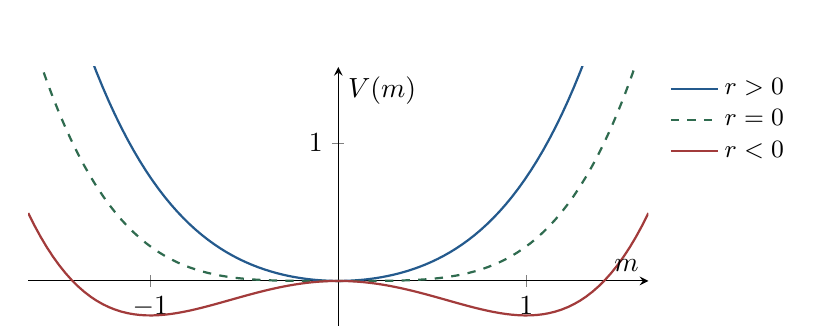
\begin{tikzpicture}
\begin{axis}[
width=0.78\textwidth,height=5cm,
axis lines=middle,xlabel={$m$},ylabel={$V(m)$},
xmin=-1.65,xmax=1.65,ymin=-0.4,ymax=1.55,
xtick={-1,0,1},ytick={0,1},
legend style={at={(1.02,1)},anchor=north west,draw=none,font=\small},
clip=true,domain=-1.65:1.65,samples=101]
\addplot[qftblue,thick] {x^2/2+x^4/4};
\addlegendentry{$r>0$}
\addplot[qftgreen,thick,dashed] {x^4/4};
\addlegendentry{$r=0$}
\addplot[qftred,thick] {-x^2/2+x^4/4};
\addlegendentry{$r<0$}
\end{axis}
\end{tikzpicture}
\caption{The quartic Landau potential with \(u=1\) and
\(r=1,0,-1\), in rescaled field units. Spin reversal is a symmetry of all
three potentials. What changes is the location and degeneracy of their
minima. These curves illustrate varying a parameter, not a computed RG
trajectory.}
\label{fig:Landau}
\end{figure}

At finite volume with \(h=0\) and symmetric boundary conditions, the exact
ensemble average \(\langle m\rangle\) vanishes because both signs occur.
Spontaneous order is defined by taking the thermodynamic limit before
removing a symmetry-breaking field, for example
\begin{equation}
m_{\rm sp}=\lim_{h\to0^+}\lim_{\mathcal V\to\infty}
\langle m\rangle_h.
\end{equation}
A saddle near one minimum describes a selected phase. Assuming
\(r\propto T-T_c^{\rm MF}\), Eq.~\eqref{eq:LandauMinima} predicts the
mean-field power \(m_{\rm sp}\propto(T_c^{\rm MF}-T)^{1/2}\).
The potential coefficients and this power are not fixed by symmetry alone.
For example, the same symmetry permits \(u<0\) with a stabilizing
\(v>0\), which can instead give a first-order transition.

For a nonuniform configuration, the saddle equation is
\begin{equation}
-\kappa\nabla^2m+rm+um^3=0.
\label{eq:statSaddle}
\end{equation}
The gradient term assigns an energy cost to domains and interfaces. On the
symmetric side, the Gaussian propagator is proportional to
\((\kappa k^2+r)^{-1}\), so the Gaussian correlation length is
\(\xi=\sqrt{\kappa/r}\). Its growth signals why fluctuations on many
length scales matter near a continuous transition.

\subsection{Coarse-grain again: the potential runs}

The choice of \(\ell\) was arbitrary. If the observer lowers the resolution
to \(b\ell\), with \(b>1\), then smaller-scale block patterns must also be
summed over. For a specified averaging map \(\mathcal B_b\),
\begin{equation}
e^{-S_{b\ell}[m']}=
\sum_{\{m_B\}:\,\mathcal B_bm=m'}e^{-S_\ell[m]}.
\label{eq:RGblocking}
\end{equation}
This is the same operation as Eq.~\eqref{eq:effectiveF}, repeated.
It preserves the partition function when the induced measure and
field-independent normalization are kept consistently. If the blocking
commutes with spin reversal, then \(S_{b\ell}[-m']=S_{b\ell}[m']\).
The symmetry survives, but the allowed coefficients change:
\begin{equation}
(r_\ell,u_\ell,\kappa_\ell,\ldots)
\longmapsto(r_{b\ell},u_{b\ell},\kappa_{b\ell},\ldots).
\end{equation}
Running here means changing the observation scale \emph{at fixed physical
temperature and microscopic Hamiltonian}. It is distinct from cooling the
magnet, which changes the microscopic Boltzmann weights.

A short calculation shows the mechanism. In the continuum, let
\(\Lambda\sim\ell^{-1}\) and split a field into slow and fast Fourier
components, \(m=\varphi+\chi\), now labeling the action by its momentum
cutoff rather than its block size. Integrate the modes with
\(\Lambda/b<|\bm q|<\Lambda\), leaving \(\varphi\) unresolved in the
partition integral. Before rescaling coordinates,
\begin{equation}
e^{-S_{\Lambda/b}[\varphi]}
=\int_{\rm shell}\mathcal D\chi\,e^{-S_\Lambda[\varphi+\chi]}.
\label{eq:RGshell}
\end{equation}
For the weakly interacting action
\(S_\Lambda=\int[\kappa(\nabla m)^2/2+rm^2/2+um^4/4]\), approximate
the fast fluctuations by the centered Gaussian quadratic theory. Their
local variance is
\begin{equation}
C_>=\langle\chi(\bm x)^2\rangle_>
=\int_{\Lambda/b<|\bm q|<\Lambda}
\frac{\dd^n q}{(2\pi)^n}\frac{1}{\kappa q^2+r}.
\label{eq:shellVariance}
\end{equation}
Assume the shell quadratic form is positive. Gaussian averaging gives
\begin{equation}
\langle(\varphi+\chi)^4\rangle_>
=\varphi^4+6\varphi^2C_>+3C_>^2.
\end{equation}
To first order in \(u\), the negative logarithm in
Eq.~\eqref{eq:RGshell} therefore produces
\begin{equation}
V_{\Lambda/b}(\varphi)
=\text{constant}+\frac12(r+3uC_>)\varphi^2
+\frac u4\varphi^4+O(u^2).
\label{eq:massRunning}
\end{equation}
The quadratic coefficient changed because unresolved fluctuations sample
the interaction. No odd term appeared. At higher orders the quartic and
other couplings change too, and derivative interactions are generally
generated. This calculation illustrates running; it is not a controlled
solution of the two-dimensional critical point.

\Needspace{10\baselineskip}
\begin{remarkbox}[An approximation that keeps only the running potential]
One can truncate the scale-dependent action to a fixed normalized gradient
term plus a general even \(V_\ell\). This is called a local-potential
approximation. It is useful because it isolates the central mechanism, but
it discards the running of the stiffness and additional derivative terms.
The potential here belongs to a partially coarse-grained action; it should
not be confused with the fully integrated Legendre effective potential,
whose convexity encodes phase coexistence.
\end{remarkbox}

\subsection{From Landau to Landau--Ginzburg--Wilson}

To compare descriptions at different cutoffs, follow the shell integration
by rescaling lengths and fields. With a canonically normalized gradient
term, Gaussian scaling assigns
\begin{equation}
[m]=\frac{n-2}{2},\qquad [r]=2,\qquad [u]=4-n.
\end{equation}
Equivalently, before fluctuation corrections, rescaling by \(b\) gives
\(r\mapsto b^2r\) and \(u\mapsto b^{4-n}u\).
For \(n<4\), the quartic interaction grows near the Gaussian fixed point:
ignoring it in the critical fluctuation problem is not self-consistent.
These are canonical scaling dimensions after field normalization, not
the engineering units of the original bounded block magnetization.

Landau's organizing idea is to identify a local order parameter, determine
how it transforms, and describe phases by the symmetry of its equilibrium
values. Ginzburg's extension retains its spatial variation. Wilson's
extension follows the whole symmetry-allowed action under coarse-graining,
rather than assuming a quartic saddle gives the final answer.

Near a continuous transition, flows can approach a scale-invariant fixed
point. Microscopic models in its basin of attraction then share
long-distance critical behavior: this is \emph{universality}. The order
parameter and its symmetries are crucial inputs, but dimension, interaction
range, other soft fields, and which fixed point is reached also matter.
Symmetry alone neither guarantees a continuous transition nor fixes its
critical exponents. The bare condition \(r=0\) is likewise a mean-field
criterion; fluctuations shift the critical surface in coupling space.

\begin{keyidea}[What this example teaches about actions]
An effective action is a record of the statistical weight left after
unobserved degrees of freedom have been summed out. Symmetry determines
which terms may occur; locality and a scale expansion organize them;
coarse-graining changes their coefficients. Landau's paradigm uses the
resulting order-parameter potential to distinguish phases. The
Landau--Ginzburg--Wilson framework also explains how their fluctuations
change with scale.
\end{keyidea}

\subsection{Return to the scalar field of Example 1}

The functional \(\int[\tfrac12(\nabla m)^2+V(m)]\) now has a microscopic
motivation. A relativistic scalar with the same internal symmetry has the
Euclidean action
\begin{equation}
S_E[\phi]=\int\dd\tau\,\dd^d x\left[
\frac12(\partial_\tau\phi)^2+\frac12|\nabla\phi|^2+V(\phi)\right].
\end{equation}
Its quadratic potential gives the free massive scalar; an even quartic term
is the leading additional polynomial interaction near four dimensions.
Formally rotating \(t=-i\tau\) relates this to the real-time scalar action,
with the appropriate analyticity and convergence prescriptions.

A classical model in \(n\) spatial dimensions is compared to a Euclidean
theory in \(n\) dimensions and, when reflection positivity and the required
continuum symmetries hold, to a quantum theory in \((n-1)+1\) spacetime
dimensions. This connection does not supply the physical relaxation dynamics
of the original magnet. The primary lesson here is the construction of an
effective action; the quantum/statistical correspondence is a consequence
to develop later.

\smallskip
\noindent\textit{Further reading:} David Tong,
\href{https://www.damtp.cam.ac.uk/user/tong/sft/}{Statistical Field Theory},
Chapters 1 and 3, for the order-parameter construction and its
renormalization-group development.

\Needspace{7\baselineskip}
\section{Questions to think about}
\begin{enumerate}
\item Derive the scalar Hamiltonian and explain why both frequency branches
in a real solution are compatible with positive energy.
\item For \(\Lag_{\rm int}=+\lambda\phi^4/4\), determine the force term and
the large-field behavior of the potential.
\item Why does a single real field with a term \(\phi\dot\phi\) fail to
produce the nonrelativistic dynamics of Eq.~\eqref{eq:NR}?
\item Derive the current in Eq.~\eqref{eq:NRcurrent}. What boundary condition
makes its integrated charge conserved?
\item Check the \(\nu=0\) and \(\nu=1\) components of
Eq.~\eqref{eq:covMaxwell} using Eq.~\eqref{eq:Fmatrix}.
\item Give an antisymmetric tensor that violates the Bianchi identity.
Which additional property of the electromagnetic field strength prevents
this?
\item Show explicitly that the source action is gauge invariant up to a
boundary term when the current is conserved.
\item For a wave moving along the \(z\)-axis, use the residual Lorenz-gauge
freedom to isolate its two transverse polarizations.
\item For a block of independent spins, derive the quadratic and quartic
terms in Eq.~\eqref{eq:entropyPotential}. Why is the action nonzero even
when the microscopic energy is zero?
\item Use the constrained sum to prove \(S_\ell[-m]=S_\ell[m]\) at zero
external field. Which terms does this symmetry forbid, and which
coefficients does it leave undetermined?
\item Explain why \(r\) can run while the microscopic temperature remains
fixed. Derive the factor \(3\) in Eq.~\eqref{eq:massRunning}.
\item What assumptions are made when only the potential is allowed to run?
Give a symmetry-allowed derivative term discarded by this approximation.
\item Distinguish symmetry of the action from symmetry of a selected
phase. Why must the thermodynamic limit precede \(h\to0\)?
\item What does the Gaussian scaling \([u]=4-n\) suggest about mean-field
theory below four dimensions? Why does symmetry alone not determine a
universality class?
\end{enumerate}

\section*{Summary}
\addcontentsline{toc}{section}{Summary}

The real scalar illustrates second-order relativistic dynamics: its modes
obey \(\omega^2=k^2+m^2\), and its Hamiltonian is positive for the free
massive theory. The complex nonrelativistic field illustrates first-order
dynamics, with \(\omega=k^2/(2M)\), a conserved norm, and a classical phase
space that should be distinguished from a one-particle state space.

Maxwell theory shows how local dynamics can be written using redundant
variables. The potential enforces the Bianchi identity, its action gives
the sourced equations, and gauge invariance requires a conserved external
current. Gauss's law is a constraint; after gauge equivalence is taken into
account, vacuum waves have two transverse polarizations.

The fourth example explains where an effective action comes from: it is
the negative logarithm of the weight obtained by summing over unresolved
microstates. Entropy generates a potential even for independent spins.
Symmetry restricts the allowed terms, and coarse-graining changes their
coefficients. Landau's paradigm distinguishes phases through a local order
parameter and symmetry breaking; the Landau--Ginzburg--Wilson framework
adds spatial fluctuations and scale dependence. A leading approximation
retains a normalized gradient term and a running even potential, while the
full action includes other running couplings as well.
\end{document}
